% =====================================================================
% Is There Exploitable Concept Drift in Industrial Tabular Data?
% A Pre-Registered Identifiability Audit
%
% TMLR submission. Source of truth for all numbers: PAPER_DRAFT_V4.md
% (v4.1, 2026-07-05) and the committed artifacts it cites
% (prereg_results/, audit_artifacts_2026-07-04/, PREREG_DEPLOYMENT_V2.md).
% Style files: official JmlrOrg/tmlr-style-file (tmlr.sty, tmlr.bst,
% fancyhdr.sty vendored alongside).
%
% Build: pdflatex main && bibtex main && pdflatex main && pdflatex main
%        (or `tectonic main.tex`, or upload the paper/ directory to Overleaf)
% =====================================================================
\documentclass[10pt]{article} % For LaTeX2e
\usepackage{tmlr}
% If accepted, instead use the following line for the camera-ready submission:
%\usepackage[accepted]{tmlr}
% To de-anonymize and remove mentions to TMLR (for example for posting to
% preprint servers), instead use the following:
%\usepackage[preprint]{tmlr}

\usepackage{amsmath}
\usepackage{amssymb}
\usepackage{graphicx}
\usepackage{booktabs}
\usepackage{array}
\usepackage{tikz}
\usetikzlibrary{shapes.geometric,arrows.meta,positioning,fit,matrix}
\usepackage{hyperref}
\usepackage{url}

% verdict marks used in Tables
\newcommand{\yes}{\checkmark}
\newcommand{\no}{$\times$}
\newcommand{\marginalmark}{$\triangle$}

\title{Label-Noise Decay Mints Concept Drift:\\
A False-Positive Channel in Loss-Based Drift Attribution,\\
and What a Certified Instrument Looks Like}

% Authors are hidden automatically while the tmlr package is used without the
% [accepted] or [preprint] options. Fill in before switching options.
\author{\name Anonymous authors \email anonymous@example.org\\
      \addr Anonymous institution}

\def\month{MM}  % Insert correct month for camera-ready version
\def\year{YYYY} % Insert correct year for camera-ready version
\def\openreview{\url{https://openreview.net/forum?id=XXXX}} % Camera-ready only

\begin{document}

\maketitle

\begin{abstract}
A drift monitor must say what moved, not merely that something did, because a changed rule P(y|x)
calls for retraining on recent data and moving covariates under a fixed rule do not. The loss-based
comparison this attribution rests on has a false-positive channel we have not found reported
elsewhere. Hold the rule provably fixed, let only label noise decay over time, and the comparison
returns a concept-drift verdict: +0.021 against a decision floor of 0.02, and within 0.003 of the
+0.024 industrial positive our own earlier instrument had reported and we had believed. Two further
channels, built adversarially against our own repair, fire the same way under fixed rules.

We then repair the instrument. Old labels are replaced by cross-fitted predictions from inside their
own window, a per-window gate flags high label noise, and the validity envelope is measured out to
the noise level at which the repaired arm itself crosses the floor on a null. A 14-cell
pre-registered battery validates the repair, including a cell where rule change and noise decay
co-occur and the repaired arm must still fire; it does, at 58\% of its clean power. Verdicts are
earned through three certificates: separability, injection, and learnability.

The repaired instrument then diagnoses the mechanism of its own earlier false positive on real
data, with the power to have seen a rule change certified in the same windows. We also measure where
it is blind, along four axes, and the last is settled from outside. Against the ACA Medicaid
expansion, a rule change documented in law, the probe read null in a fully identifiable regime and
at the tightest detectable bound in the paper, because its score is rank-based and an eligibility
threshold moves mass across a decision boundary without reordering anyone.

On eight industrial datasets (TabReD), with a fresh-seed replication that leaves 10 of 10 verdicts unchanged, it finds
no exploitable mean-rule drift above each dataset's detectable floor for the deployed tree-ensemble
class: 0/8 audited, 0/5 among the cells that carry an informative reading. A frame that does attribute shift types, run head-to-head on the same battery, separates
the two mechanisms by magnitude but not by sign, so a threshold reading files two events with
different repairs as one. We release the instrument, the battery and the audit trail, and argue that
drift-type attribution without identifiability certificates, the current default, is unreliable.
\end{abstract}

\section{Introduction}\label{sec:intro}

A team watching a deployed tabular model sees its recent loss rise and has to choose. Retrain on
recent data only, discarding older rows as stale, which is right if the labeling rule has changed.
Or keep everything, because the rule is intact and the older rows still carry correct labels, which
is right if only the covariates moved. Choosing wrongly is expensive in both directions, and
choosing is what drift-type attribution is for.

The comparison that attribution usually rests on is simple enough to be trusted without checking:
fit a model on recent data, fit another on recent plus old data, and read the gap on a future
window. If old rows now mislead, adding them hurts. We call this quantity \emph{staleness harm}, and it
is deployment-native in a way importance-weighted decompositions are not. The recent portion is
identical in both arms, so covariate coverage cancels by construction, and nothing needs density
ratios or overlapping supports, which is exactly what fails in industrial feature spaces.

\textbf{The comparison has a false-positive channel.} Its informal justification, that correct labels cannot
hurt, is false for finite-capacity empirical risk minimization. Hold the rule provably fixed, let
only the \emph{noise} on the labels decay over time, and the comparison fires: unweighted ERM is not
efficient under heteroscedasticity, so noisier old rows inflate the loss of any model that fits
them, and removing them improves recent-window loss for reasons that have nothing to do with the
rule. On a constructed null this reads +0.021, above the 0.02 floor this literature's thresholds live
near and within 0.003 of +0.024, an industrial positive our own v2 instrument had reported and we
had believed. A monitor consuming that number would retrain on recent data and
throw away correct labels, while telling its owners the rule had changed. Two further channels,
constructed adversarially against our own repair, fire the same way: x-dependent noise whose scale
decays (+0.025), and noise correlated with the rule-carrying feature (+0.026), the denoiser's worst
case. Growing noise reads $-0.023$, so the artifact is directional rather than a constant bias.

\textbf{Two more ways the naive instrument lies}, repaired in Section~\ref{sec:certificates} and mapped in Section~\ref{sec:classrel} respectively. The
natural certificate for ``a null here is uninformative'' is a window-separability AUC, which asks
whether a classifier can tell old rows from future rows. Computed row-wise it saturates to
0.994--1.000 under exact duplicates, near-duplicates and entity cohorts with no covariate shift at
all: the classifier memorizes rows, not distributions, and
eight of ten real datasets read exactly 1.000 under the naive gate. And the concept/covariate
separation is hypothesis-class-relative: a kNN probe reads pure covariate shift as concept drift
(+0.098) and a two-layer MLP reads fixed-rule prior shift as concept drift (denoised +0.042), while
tree ensembles pass all controls. That is Shimodaira's misspecification result made empirical, and
it means ``old data hurts'' can be manufactured by geometry alone.

\textbf{The repair, and the discipline it needs.} Each failure gets a repair validated by execution
(Section~\ref{sec:instrument}--Section~\ref{sec:validation}). A \emph{denoised staleness} arm replaces old labels with cross-fitted predictions from inside
their own window: under noise-only drift those pseudo-labels are approximately correct and the harm
vanishes, while under a changed rule they still encode the old rule and the harm persists. A
per-window noise gate flags the confound, and its validity envelope is measured rather than assumed,
out to the noise level at which the denoiser itself crosses the decision floor on a null; beyond
that the instrument abstains. A group-aware separability estimate deflates memorization while
leaving honest drift intact. And learnability-gated injection controls turn "this dataset is
unmeasurable" from an assumption into a demonstration. All verdicts are scoped to the tree-ensemble class, with linear and kNN
probes carried as canaries whose false fires are reported rather than hidden.

\textbf{The instrument turned on itself.} Pointed back at the dataset that produced our prior positive,
the repaired instrument reproduces the v2 raw reading bit-for-bit, measures old-window label noise
at 2.1--2.9$\times$ the recent median, and returns a \emph{significantly negative} denoised arm at every window
resolution: with the noise removed the old rows help. The same windows recover a rule planted at
reference strength (+0.086, learnable at R$^2$ 0.93), so the negative is certified rather than
argued. We are not aware of a prior case of a drift-attribution instrument diagnosing the
\emph{mechanism} of its own earlier false positive on real data, as opposed to failing to replicate it.

\textbf{And its blind spots, measured.} A null is worth its blind spots, so we map ours (Section~\ref{sec:blind}) along four
axes: probe class, separability, rule family, and metric. The last is settled from outside. The ACA
Medicaid expansion, implemented by Pennsylvania on 2015-01-01 and never adopted by Texas, is a rule
change documented in law and visible in the raw positive rates (0.234 $\to$ 0.306 against a flat
0.183--0.185). The probe read both states null, in a fully identifiable regime and at the
tightest detectable bound anywhere in this paper, so a confident zero rather than an underpowered
one. The mechanism was registered before the run: our binary score is AUC, which is rank-based, and
an eligibility threshold moves a large mass across a decision boundary without reordering anyone.
Under proper scores the same windows turn positive on the treated state (+0.021 under log-loss)
against +0.006 on the control. That localises the blindness and gives a repair direction, and Section~\ref{sec:metricrel}
states the three things the reading does not license.

\textbf{The application.} With the instrument certified and its blind spots mapped, we spend it on the
question that motivated building it (Section~\ref{sec:application}): a pre-registered audit of eight TabReD datasets,
Electricity and the INSECTS streams, with confirmatory fresh-seed replication (10/10 stable). The
result is an identifiability map rather than a detection table: 0/8 audited and 0/5 among the cells
that carry an informative reading, the sole robust positive being designed drift, with two cells
refusing a certificate outright rather than counting as evidence and one already diagnosed in
Section~\ref{sec:diagnosis}. Anchor streams fix the
sensitivity profile: monotone and single-switch rule changes fire 9/9, and recurring regimes are
correctly silent with a negative-recency fingerprint that is impossible under one-way drift.

\textbf{Contributions.}

\begin{enumerate}
\item \emph{A false-positive channel in loss-based drift attribution} (Section~\ref{sec:channel}), executed rather than argued:
label-noise decay under a provably fixed rule mints concept verdicts at magnitudes matching real
borderline positives, with two further channels found by adversarial construction, and a
head-to-head showing a type-attributing frame separates the mechanisms by magnitude but not by
sign.
\item \emph{A repaired, abstaining instrument} (Section~\ref{sec:instrument}--Section~\ref{sec:validation}): denoised staleness with a noise gate and a measured
validity envelope, group-aware separability, learnability-gated injection certificates,
class-scoped verdicts with canaries, validated on a 14-cell pre-registered battery including
the adversarial combination in which rule change and noise decay co-occur (fires at 58\% of
clean power).
\item \emph{A measured map of an instrument's blind spots} (Section~\ref{sec:blind}), including one settled against external
ground truth: class relativity (a linear monitor flips the canonical Electricity dataset to
concept drift on identical bytes), continuous power collapse inside the separability gate
($\rho$ = $-0.47$), family relativity (a subpopulation-local rule learnable at R$^2$ 0.560 and
unrecovered at $-0.050$), and metric relativity (the ACS falsification).
\item \emph{A pre-registered identifiability map of industrial tabular ML} (Section~\ref{sec:application}): 0/8 audited and 0/5
informative, one diagnosed false positive with mechanism, per-dataset certificates and
detectable-effect bounds, 10/10 confirmatory stability and 10/10 cross-class agreement.
\end{enumerate}

\textbf{What we do not claim.} We do not claim concept drift is absent from industrial tabular data:
several cells are certified \emph{blind}, and blindness is not absence. We do not claim the
identifiability theory is new: that overlap failure blocks nonparametric identification is
classical, and class-relativity is established. Our contribution is the executed channel, the
repaired instrument, and the certified map. We do not claim model-agnosticism: every verdict is
relative to the deployed hypothesis class, which we argue is the only honest way to state
drift-type attribution at all. We do not claim the noise channel is the only way this comparison
fails, only that it is one nobody had reported and that it is large enough to have fooled us. And
we do not claim our own instrument is trustworthy everywhere. Section~\ref{sec:blind} is the list of places where it is
not, and one entry on that list was set by a state's policy decision rather than by us.

\section{Related Work}\label{sec:related}

\paragraph{Shift-type maps on tabular data.} WhyShift \citep{liu2023whyshift} is the closest prior: it
attributes performance drops to $Y \mid X$- vs $X$-shift across tabular datasets and concludes
$Y \mid X$-shifts are prevalent---on predominantly spatial/subpopulation axes, under an
overlap-assuming decomposition. Our delta is threefold: the \emph{temporal} axis on deployed
industrial representations (where positivity actually fails and their lens degenerates), an
\emph{abstention arm} with per-dataset certificates (WhyShift assumes the decomposition is
measurable), and the instrument-failure anatomy. DISDE \citep{cai2023disde} supplies the
decomposition formalism we inherit terminology from; its shared-distribution term is identified
only on common support---the boundary our map makes operational. TabReD itself
\citep{rubachev2025tabred} frames everything as ``gradual temporal shift'' and contains no
decomposition or recency experiments; TableShift \citep{gardner2023tableshift} and Wild-Time
\citep{yao2022wildtime} are shift benchmarks without drift-type attribution.

\paragraph{Identifiability and class-relativity.} That $P(y \mid x)$ is not identified off-support without
assumptions is textbook positivity (\citealp{damour2021overlap}, for high-dimensional overlap
failure; \citealp{bendavid2010impossibility}, for the learning-theoretic impossibility;
\citealp{johansson2019support}, for support failure inside learned representations).
\citet{hinder2023hardness} prove constructively that loss-based drift detection is class-relative
in both directions---virtual drift that moves the loss, real drift invisible to it---and their
survey \citep{hinder2024survey} states ``the used model class is crucial.'' \citet{loog2019minimizers}
show ERM risk can be non-monotone in sample size even i.i.d., closing the door on any
unconditional ``more correct data cannot hurt'' lemma. \citet{gowerwinter2026window} argue drift
detection is ill-posed through windowing choices. We treat all of this as settled theory that the
applied drift-monitoring stack has not absorbed, and contribute the executed demonstration $+$ the
repaired protocol; we state no theorems of our own---where the paper sounds formal (the
envelope, the certificates), the content is a measured boundary, not a proved one.

\paragraph{Old data harming.} \citet{shimodaira2000improving} is the mechanism for the misspecified case;
the Data Addition Dilemma \citep{shen2024data} documents mixture harm empirically in clinical ML;
\citet{klinkenberg2000detecting} use held-out error over candidate training windows to \emph{adapt}
window size. We are not aware of prior work that uses the add-old-data contrast as a
drift-\emph{type} identifier with verdict semantics, or that reports the label-noise-decay
false-positive channel---under the field-standard definition of real drift as any change in
$P(y \mid x)$ \citep{gama2014survey,webb2016characterizing}, noise drift \emph{is} drift, which is precisely why an
instrument that claims to detect \emph{exploitable rule change} must separate the two; we separate
them by construction and validate the separation adversarially.

\paragraph{Pseudo-labels, denoising, cross-fitting.} The denoised arm's mechanics are deliberately
borrowed: replacing labels with model predictions is self-training \citep{scudder1965probability,lee2013pseudolabel}
and distillation \citep{hinton2015distilling}; the view of noisy labels as recoverable by a fitted
model underlies noisy-label learning \citep{natarajan2013noisy,han2018coteaching}; strictly
out-of-fold prediction to avoid own-fit contamination is cross-fitting \citep{chernozhukov2018double}.
What we take from these literatures is the estimator; the \emph{use}---as the discriminating
arm of a drift-type verdict, with an adversarially mapped validity envelope and an abstention
rule---is the contribution we claim, and we scope it to its evidence: none of these adjacent
literatures, to our reading, reports the failure channel this arm exists to defuse.

\paragraph{Drift detectors and their evaluation.} Classical detectors \citep[surveys:][]{gama2014survey,lu2019learning}
monitor loss or distribution statistics and are evaluated by injecting known drifts
into streams \citep{poenaruolaru2022reliable}; Detectron \citep{ginsberg2023detectron} defines harmful
shift model-relatively. Our injection control differs in role: it is an \emph{in-situ, per-dataset
power certificate} (planted in the real covariate geometry, learnability-gated), used to
distinguish earned blindness from instrument vacuity---a distinction we show matters on real
data, where \emph{all four} of the industrial ``unidentifiable'' cells fail to earn a certificate
(three because the planted rule is unlearnable in their geometry, the fourth because its
learnability score straddles the gate across seed sets). We do not run
these detectors head-to-head on the audited cells: a loss-stream detector answers ``did anything
change?'' and is type-blind by construction, so its fires would not bear on drift-\emph{type}
attribution; the canary panel (\S\ref{sec:classmatrix}) is the like-for-like comparison---what a
weaker \emph{attribution} instrument reports on the same bytes---and porting the certificate
protocol to streaming monitors is future work (\S\ref{sec:discussion}).

\paragraph{Malware.} TESSERACT \citep{pendlebury2019tesseract} established temporally honest evaluation in
malware and documents performance decay. Our EMBER read (old data \emph{helps}; staleness $-0.008$;
detectable floor 0.0013) refines rather than contradicts it: the decay is coverage-driven (new
families appear---covariate expansion), not label rot (a 2017 malware sample is still malware),
which is exactly the distinction a deployment lens should draw.

\section{The Instrument}\label{sec:instrument}

\begin{figure}[t]
\centering
\resizebox{\textwidth}{!}{\input{figures/fig1_cascade_body}}
\caption{The decision cascade of the instrument. The cascade is specified verbatim in
\S\ref{sec:cascade} and PREREG \S3. Side channels attached to every run: the strict-rule shadow
verdict (rule-sensitive flag), the negative-recency fingerprint for recurring regimes
(\S\ref{sec:anchors}), the canary-probe panel (\S\ref{sec:classmatrix}), and provenance stamping
on every run.}
\label{fig:cascade}
\end{figure}

\emph{Reading aid.} One real cell exercises most of the vocabulary in Table~\ref{tab:terms}. On
sberbank-housing (\S\ref{sec:diagnosis}), the raw arm fires ($+0.024$) but the noise gate is on
($2.1\times$) and the denoised arm is negative---so the cascade returns NOISE-DRIFT-CONFOUNDED
rather than concept; had all three aligned inside the envelope, the verdict would have been
DEPLOYMENT-CONCEPT, subject to an injection positive control.

\begin{table}[t]
\caption{Terminology (one line each).}
\label{tab:terms}
\centering
\footnotesize
\begin{tabular}{@{}l>{\raggedright\arraybackslash}p{4.55in}@{}}
\toprule
term & meaning \\
\midrule
raw staleness & future-window score(recent) $-$ score(recent $\cup$ old); $>0$ = old data hurts \\
denoised staleness & same, with old labels replaced by cross-fitted within-old-window predictions; $>0$ = the \emph{rule} changed \\
noise gate & old-window noise proxy / recent median; $>1.5$ = label-noise drift present \\
envelope & noise-ratio 4.7, the measured boundary of denoiser validity; above it the instrument abstains \\
$D$ & window-separability AUC (group-aware, size-matched); a routing statistic, \emph{not} support overlap \\
injection & a known rule rotation planted in the dataset's own geometry; the per-dataset power certificate \\
earned blindness & injection learnable in-window yet unrecoverable $\to$ the geometry genuinely hides this signal class \\
injection-vacuous & injection unlearnable $\to$ the null certifies nothing \\
no-evidence band & sub-floor CI-positive readings; calibrated on no-drift anchors as noise \\
canary probe & a deliberately misspecified probe class (linear/kNN) whose false fires are reported \\
rule-sensitive & verdict differs between the primary and strict decision rules; barred from headlines \\
\bottomrule
\end{tabular}
\end{table}

\subsection{Setting and estimand}\label{sec:setting}

Rows $(x_i, y_i, t_i)$ arrive over time; the auditor sees the full labeled history (retrospective
audit, not online prediction). Fix $K$ windows by timestamp-value rank (ties never straddle
boundaries; per-seed boundary jitter). For each future window $W_j$ (back half), with old anchor
$W_0$ (earliest window with $\ge 200$ rows and a trainable label set) and recent window $W_{j-1}$, draw
size-matched samples ($N = \min(|\text{recent}|, |\text{old}|, 6000)$) and train three models of the deployed
class: recent-only, old-only, recent$\,\cup\,$old. Report per-seed means over future windows of
\begin{itemize}
\item \textbf{decay} $=$ score(old model, held-out $W_0$) $-$ score(old model, $W_j$)---aging,
  mechanism-blind (documented at scale by \citealp{vela2022temporal});
\item \textbf{recency gain} $=$ score(recent) $-$ score(old) on $W_j$---adaptation value, conflates coverage
  and rule change; \emph{its sign is itself diagnostic (\S\ref{sec:anchors}): negative recency is impossible under
  one-way drift and fingerprints recurring regimes};
\item \textbf{raw staleness} $=$ score(recent) $-$ score(recent$\,\cup\,$old) on $W_j$---the attribution probe;
\item \textbf{denoised staleness} $=$ score(recent) $-$ score(recent $\cup$ $(X_{\text{old}}, \hat{g}_{\text{old}}(X_{\text{old}}))$) on $W_j$, where
  $\hat{g}_{\text{old}}$ is a 2-fold cross-fitted model \emph{within} $W_0$ producing strictly out-of-fold hard
  pseudo-labels.
\end{itemize}
Scores: AUC (binary), accuracy (multiclass), $-$RMSE on z-scored targets (regression). CIs are
Student-$t$ over 10 seeds; each seed re-draws a 90\% row subsample, re-jitters window boundaries,
and re-samples all training sets. These are seed-level intervals over heavily overlapping
subsamples and are anti-conservative for tiny effects (\S\ref{sec:anchors} calibrates the resulting no-evidence
band on no-drift anchors); verdict-level inference does not rest on them alone---the
confirmatory fresh-seed replication (\S\ref{sec:protocol}) is the operative stability check, and per-seed values
are emitted with every run so that alternative constructions (window-block bootstrap, split-half)
can be applied without re-execution. The pre-registered estimand is \emph{exploitable mean-rule drift}:
a change in the decision-relevant functional of $P(y \mid x)$ that makes old labels contradict the
current rule for the deployed hypothesis class. This is deliberately narrower than the
field-standard ``any change in $P(y \mid x)$'' \citep{morenotorres2012unifying,webb2016characterizing}---the narrowing is the point, because
the wider definition classifies label-noise drift as concept and thereby licenses retraining
that cannot help.

\paragraph{Why the denoised arm separates rule change from noise drift.} Under noise-only drift the
conditional mean/Bayes rule is unchanged, so $\hat{g}_{\text{old}}$ estimates the \emph{same} rule from noisy labels;
its pseudo-labels are approximately correct denoised labels, and adding $(X_{\text{old}}, \hat{g}_{\text{old}}(X_{\text{old}}))$
to the recent set has no remaining mechanism to hurt through (an expectation whose boundary
\S\ref{sec:envelope} measures, not a theorem)---executed: the $+0.021$ noise-decay false positive
collapses to $+0.004$ while the gate (below) flags the mechanism. Under genuine rule change,
$\hat{g}_{\text{old}}$ consistently estimates the \emph{old} rule; its pseudo-labels still contradict the current
rule, and the harm persists---executed: a rotating-rule stream keeps $+0.541$ of its $+0.546$ raw
signal, and rule-change-plus-noise-decay still fires at $+0.316$. The denoiser is not unbiased:
its pseudo-label error grows with old-window noise, and we \emph{mapped the boundary}---at an
old/recent noise ratio $\approx 5.7$ the denoised arm itself crosses the decision floor on a pure null
($+0.026$). The instrument therefore carries an envelope constant (abstain above ratio 4.7) rather
than a pretense of a theorem; per \citet{loog2019minimizers}, no unconditional soundness lemma exists to
be had.

\paragraph{The noise gate.} Per window, a fresh model of the deployed class is fit on 70\% and its
held-out irreducible-error proxy recorded (regression: MSE on z-scored $y$; binary: $1-$AUC;
multiclass: $1-$accuracy). The gate statistic is old-window proxy / median recent-window proxy;
it fires above 1.5 (stable synthetic controls calibrate at 0.75--0.99) and defines the envelope
above 4.7. The gate alone is \emph{not} a sufficient repair---a gate-veto rule would misfile genuine
rule change co-occurring with noise drift (executed: $+0.316$ must fire despite gate 3.67)---it
supplies the \emph{mechanism label} (NOISE-DRIFT-CONFOUNDED) when the raw arm fires and the denoised
arm does not.

\subsection{Certificates: separability, injection, learnability}\label{sec:certificates}

\paragraph{Window separability $D$ (not ``overlap'').} $D$ is the median held-out AUC of a classifier
separating $W_0$ from each back-half window, on the proxy-stripped feature space, with two
repairs over the naive version: size-matching by \emph{random subsample} (a head-slice on
time-sorted rows manufactures separability from window-size imbalance---executed: shuffle-$D$
0.94 with no static feature, collapsing to 0.50 under the fix) and a \emph{group-aware} train/test
split keyed on near-duplicate clusters (z-scored rows rounded to 0.1): exact duplicates at
multiplicity 5 inflate row-split $D$ to 0.994 and entity cohorts to 1.000 with zero covariate
shift; the group split returns both to $\approx 0.50$ while honest drift keeps $D$ high. We report $D$ as
\emph{separability}, never as support overlap: a single genuinely predictive drifting feature
saturates it, so $D \ge D^{\ast} = 0.96$ routes a staleness null to the injection control rather than
concluding anything by itself.

\paragraph{Learnability-gated injection.} For any candidate-unidentifiable dataset (and, as a positive
control, for any CONCEPT verdict), a reference concept---a rule rotation of fixed strength on
the two highest-variance features---is planted in the dataset's own $(X, t)$ geometry and the full
staleness pipeline re-run (10 seeds, same power as the main read). Before the null is allowed to
mean anything, the injected rule must be \emph{learnable in-window} (held-out AUC $\ge 0.65$ / $R^2 \ge 0.20$
/ accuracy $\ge$ majority $+\ 0.10$): executed on a constructed geometry whose top-variance features
are heavy-tailed junk, the injected rule is unlearnable (in-window AUC 0.506) and the naive
protocol grants ``earned blindness'' vacuously; the gate converts that to \emph{injection-vacuous}---%
certificate refused. Outcomes: recovery ($\Rightarrow$ the real null was informative: verified no-concept),
earned blindness (learnable but unrecoverable $\Rightarrow$ the geometry genuinely hides this signal
class), or vacuity (no certificate). On the real audit, this distinction is load-bearing: all four
``unidentifiable'' industrial cells, two fail the learnability gate under every signal family
tried and end with no certificate; the other two resolve only once the family is widened
---\texttt{homesite\_insurance} scores within 0.05 of the gate on the reference family and flips
across seed sets, but is comfortably learnable and consistently unrecovered on the low-variance
one, and weather is unlearnable on the reference family yet recovers on two others
(\S\ref{sec:results}). The certificate is explicitly
relative to this reference family: recovery certifies power against rotations carried by the
dataset's high-variance directions, not against rule changes living in low-variance features,
interactions, or subpopulations (\S\ref{sec:discussion}, Limitation 6).

\paragraph{The identification boundary (restatement of prior work, not a new result).}
Let $R$ be the region of covariate space the future windows occupy and the old anchor does not. On
$R$, $P(y \mid x)$ is not nonparametrically identified from the observed windows: two conditionals
that agree on the old window's support and differ on $R$ induce identical observable data, because
no old rows fall in $R$. This is the time-axis instance of the shared-support requirement that
DISDE makes explicit \citep[Prop.~1]{cai2023disde}, and we claim no theorem of our own. Three
properties of the instrument follow from it rather than from convenience. Abstention is
\emph{correctness}, not timidity. $D$ is a routing statistic for how close a panel sits to that
boundary, and never a measure of support overlap itself---which is why $D \geq D^\star$ concludes
nothing on its own and hands off to the injection control. And a cell without an identifiability
certificate cannot be evidence of \emph{no drift}; it is only evidence of \emph{no measurement},
which is why we carry the 0/5 certified count alongside the pre-registered 0/8
(\S\ref{sec:results}). In the opposite direction---\emph{soundness}, i.e.\ staleness $>0$ implying
rule change---no theorem is available to be had: \citet{loog2019minimizers} show ERM risk is
non-monotone in added same-distribution data, so $\mathbb{E}[\text{staleness}] > 0$ is possible
under zero drift and zero heteroscedasticity. That asymmetry is why \S\ref{sec:envelope} reports a
\emph{measured} validity envelope where a soundness lemma would otherwise go.

\subsection{Decision cascade and scope}\label{sec:cascade}

The pre-registered cascade (PREREG \S3; verbatim in the artifact): DEPLOYMENT-CONCEPT requires
the \emph{denoised} arm to fire (CI lower bound $> 0$ and mean $> 0.02$) within the noise envelope; a raw
fire with the gate on is NOISE-DRIFT-CONFOUNDED; a raw fire with the gate off is
RAW-ONLY-POSITIVE (unresolved, never concept); nulls route through $D$ to the injection
certificates; a sub-floor denoised CI is reported as a no-evidence band (calibrated: 2/5 no-drift
anchor streams land there at 1/10--1/20 of the floor---CI-significant, decision-irrelevant). A
strict secondary rule (CI lower bound $>$ floor) is computed alongside; any cell whose verdict
differs between the two readings is marked rule-sensitive and barred from headlines. Every
verdict is scoped to the deployed hypothesis class: the ground-truth suite passes under HGB and
random forests and fails under linear/kNN probes (\S\ref{sec:validation}), so tree-ensemble verdicts are
decision-grade and linear/kNN run as canaries. All runs emit provenance metadata (commit, argv,
library versions, seeds) into versioned artifacts; the decision rules, thresholds, seed
protocol (exploratory 0--9, confirmatory 100--109), and aggregate reading were committed before
the runs they govern. Appendix~\ref{app:constants} tabulates every decision constant with its
calibration source and validity range.

\section{Validation: the battery, the envelope, and the class matrix}\label{sec:validation}

\subsection{The 14-cell pre-registered battery}\label{sec:battery}

The instrument must pass a synthetic ground-truth battery before any real-data run (PREREG \S4);
the battery is itself the executed record of the failure anatomy. All cells: $n = 12{,}000$, $d = 10$,
$K = 10$, 5 seeds (vs ten on real data---the planted effects are 10--27$\times$ the decision
floor and the battery is a pass/fail gate, not an estimation exercise); verdicts under the full
cascade (Table~\ref{tab:battery}).

\begin{table}[t]
\caption{The 14-cell pre-registered battery. Verdicts under the full cascade; all cells
$n = 12{,}000$, $d = 10$, $K = 10$, 5 seeds.}
\label{tab:battery}
\centering
\footnotesize
\setlength{\tabcolsep}{4pt}
\begin{tabular}{@{}>{\raggedright\arraybackslash}p{2.0in}rrr>{\raggedright\arraybackslash}p{2.35in}@{}}
\toprule
cell (truth) & raw & denoised & gate & verdict \\
\midrule
rotating rule (binary) & $+0.280$ & $+0.289$ & 0.90 & \textbf{CONCEPT}~\yes \\
rotating rule + drifting nuisance & $+0.203$ & $+0.206$ & 1.18 & \textbf{CONCEPT}~\yes\ (proxy-stripped) \\
rotating rule (regression) & $+0.546$ & $+0.541$ & 0.91 & \textbf{CONCEPT}~\yes \\
\textbf{rotating rule + noise decay} & $+0.357$ & $\boldsymbol{+0.316}$ & 3.67 (fires) & \textbf{CONCEPT}~\yes---the gate must not veto \\
covariate shift, fixed rule & $-0.001$ & $-0.000$ & 0.74 & UNIDENT (blindness earned)~\yes \\
stationary & $-0.001$ & $-0.000$ & 0.75 & NO-STRONG-CONCEPT~\yes \\
prior shift, fixed rule (multiclass) & $-0.003$ & $-0.004$ & 0.84 & UNIDENT, injection-vacuous~\yes \\
mild covariate shift ($D = 0.73$, un-gated) & $-0.003$ & $+0.001$ & 0.99 & NO-STRONG-CONCEPT~\yes---the null is load-bearing, not gated away \\
stationary (regression) & $-0.012$ & $-0.002$ & 0.99 & NO-STRONG-CONCEPT~\yes \\
covariate shift, fixed \emph{linear} rule (reg.) & $+0.002$ & $+0.004$ & 0.91 & UNIDENT~\yes\ (never CONCEPT) \\
covariate shift, fixed \emph{nonlinear} rule (reg.) & $-0.005$ & $-0.003$ & 0.92 & UNIDENT~\yes \\
\textbf{label-noise decay, fixed rule} (the F1 killer) & $\boldsymbol{+0.021}$ \textbf{fires} & $+0.004$ & 3.54 & \textbf{NOISE-DRIFT-CONFOUNDED}~\yes \\
label noise \emph{growing}, fixed rule & $-0.023$ & $-0.019$ & 0.14 & NO-STRONG-CONCEPT~\yes \\
\textbf{$x$-dependent noise, decaying scale} & $\boldsymbol{+0.025}$ \textbf{fires} & $+0.005$ & 3.76 & \textbf{NOISE-DRIFT-CONFOUNDED}~\yes \\
\bottomrule
\end{tabular}
\end{table}

Three cells carry the paper's argument. The noise-decay cell is the executed refutation of
``correct labels cannot hurt'': the raw probe fires at a magnitude ($+0.021$) that matched a real
industrial positive to within 0.003. The $x$-dependent-noise cell is a \emph{second} raw false-positive
channel, discovered during adversarial review of the repair itself; a third (noise scale
correlated with the rule feature---the denoiser's worst case, since pseudo-label error then
concentrates where the signal lives) was constructed by an independent red-team pass and also
defused (raw $+0.026$ fires; denoised $+0.006$, null). The concept-plus-noise cell establishes that
the repair keeps power where both mechanisms co-occur: denoised retention is 58\% of the clean
rotating-rule signal ($+0.316$ vs $+0.541$), and the same holds at small rule-change magnitudes
(a 0.8-rad rotation: clean denoised $+0.108$, with noise decay $+0.062$---attenuated, still firing).
Robustness of the denoiser to a small old window was checked directly (old window capped at 600
rows, cross-fit folds of 300): no false positive ($+0.004$) and no false negative ($+0.429$).

\paragraph{Floor comparability across metrics.} The 0.02 decision floor is shared across AUC, accuracy,
and z-scored $-$RMSE, which are not decision-equivalent units. Two mitigations are structural:
every null carries its own detectable-effect bound $\delta$ (the per-dataset, per-metric power
statement that does the aggregate's real work), and CONCEPT never rests on the floor alone (the
denoised CI, gate, and envelope must all align). As a sensitivity check, re-thresholding all
committed runs under per-metric floors rescaled by the battery's matched-strength concept
magnitudes (binary $+0.28$ vs regression $+0.55$ $\Rightarrow$ regression floor 0.04) moves no cell across the
concept/no-concept boundary; the only affected cell is the mechanism label of the diagnosed
regression positive (\S\ref{sec:diagnosis}), which is already flagged rule-sensitive and barred from headlines.

\subsection{The envelope: where the repair itself breaks}\label{sec:envelope}

The denoiser is biased---pseudo-label error grows with old-window noise---and rather than
assuming the bias negligible we mapped it: on pure fixed-rule nulls, the denoised arm reads
$+0.0037$ at noise-ratio 3.54, $+0.0048$ at 3.76, $+0.0043$ at 3.87, $+0.0140$ at 4.72, and \textbf{$+0.0259$ at
5.71---across the 0.02 decision floor on a null}. The instrument therefore abstains
(NOISE-AMBIGUOUS) above ratio 4.7. Separation still exists beyond the envelope (at ratio $\approx 6$, a
true rotating rule reads denoised $+0.086$ vs the null's $+0.026$, disjoint CIs), but any threshold
there would be calibrated on a single noise family, so we refuse the verdict instead. Stable
controls calibrate the gate statistic at 0.75--0.99, far from the 1.5 firing threshold; every
real-data gate value in \S\ref{sec:map} falls either clearly below 1.5 or in 2.0--2.9---nowhere near the
envelope edge.

\subsection{The model-class matrix: why verdicts are class-scoped}\label{sec:classmatrix}

Re-running the five core controls with the probe's model class swapped (the instrument's every
component---staleness arms, gate, separability, injection---follows the swap) yields
Table~\ref{tab:classmatrix}.

\begin{table}[t]
\caption{The model-class matrix: the five core controls with the probe's model class swapped.}
\label{tab:classmatrix}
\centering
\footnotesize
\setlength{\tabcolsep}{3.5pt}
\begin{tabular}{@{}>{\raggedright\arraybackslash}p{1.05in}>{\centering\arraybackslash}p{0.72in}>{\centering\arraybackslash}p{0.85in}>{\centering\arraybackslash}p{1.15in}>{\centering\arraybackslash}p{1.05in}>{\centering\arraybackslash}p{1.05in}@{}}
\toprule
control (truth) & HGB & RandomForest & MLP (64,32) & linear & kNN \\
\midrule
rotating rule & \yes\ ($+0.280$) & \yes\ ($+0.287$) & \yes\ ($+0.305$) & \yes\ ($+0.310$) & \yes\ ($+0.295$) \\
covariate shift, fixed rule & \yes\ ($-0.001$) & \yes\ ($+0.004$) & \marginalmark\ (den $+0.045$, CI-saved) & \yes\ ($-0.002$) & \textbf{\no\ CONCEPT ($+0.098$)} \\
prior shift, fixed rule & \yes\ ($-0.003$) & \yes\ ($+0.003$) & \textbf{\no\ CONCEPT (den $+0.042$)} & \textbf{\no\ CONCEPT ($+0.026$)} & \textbf{\no\ CONCEPT ($+0.048$)} \\
stationary & \yes & \yes & \yes & \yes & \yes \\
rotating rule + nuisance & \yes\ ($+0.203$) & \yes\ ($+0.200$) & \yes\ ($+0.228$) & \yes\ ($+0.229$) & \yes\ ($+0.219$) \\
\bottomrule
\end{tabular}
\end{table}

Concept \emph{detection} is class-robust (all five classes fire on true rotations); the
concept/covariate \emph{separation}---the property the verdict rests on---holds only for classes
flexible enough to represent the fixed rule. This is \citet{shimodaira2000improving} made empirical: under
misspecification the mixture-ERM optimum moves with $P(x)$, so covariate shift alone manufactures
``old data hurts.'' Denoising does not repair this channel (kNN still false-fires at $+0.111$ with
pseudo-labels---the misspecification is in the \emph{probe}, not the labels), which is why the
instrument's verdicts are stated as tree-ensemble-scoped, with linear/kNN carried as canaries.
The neural probe deserves emphasis, because the paper's motivating question is whether deep
tabular architectures have a rule change to exploit: \textbf{a two-layer MLP probe fails the
separation battery}---it reads fixed-rule prior shift as concept drift (denoised $+0.042$, a
fire) and leans positive on pure covariate shift (denoised $+0.045$, saved only by CI width)---so
it joins the canaries rather than the decision-grade classes. We do not claim this extrapolates
to modern deep tabular architectures at scale; we claim the direction of the burden: a probe
class earns drift-verdict authority by passing this battery, and the first neural probe we
tested does not. The practical reading for the field is uncomfortable: \textbf{a drift monitor built
on a linear, local, or small-neural probe can report concept drift on data where a
tree-ensemble monitor reports none, on the same bytes}---and \S\ref{sec:classpanel} shows this happens on the
canonical real drift dataset, not just in synthetics.

\section{The Map}\label{sec:map}

\subsection{Protocol}\label{sec:protocol}

Eight TabReD datasets \citep[train segments of the official temporal splits]{rubachev2025tabred},
Electricity (elec2), and INSECTS (incremental-balanced)---HGB probe, $K = 10$, 10 exploratory
seeds (0--9), then a \textbf{confirmatory rerun with fresh seeds (100--109)}; any verdict that moves
between the two is reported unstable and barred from claims. Decision cascade, thresholds, seed
protocol, and the aggregate reading were committed before execution; the prior (v2-era)
industrial positive was pre-registered as a \emph{retraction candidate with a prediction}
(NOISE-DRIFT-CONFOUNDED or denoised-null), and a survival battery was pre-specified in case the
prediction failed. Both the primary rule (CI $> 0$ $\wedge$ mean $>$ floor) and the strict rule
(CI $>$ floor) are computed; rule-sensitive cells are flagged.

\subsection{Results: 10/10 confirmatory-stable; industrial mean-rule drift 0/8 audited, 0/5 certified}\label{sec:results}

\begin{figure}[t]
\centering
\resizebox{\textwidth}{!}{% Figure 2 body — the identifiability map at a glance (PAPER_DRAFT_V4 §5.2, Table 4 rendered).
% Single source of the tikzpicture. Consumers: ../main.tex (\input) and fig2_map.tex (standalone).
% Numbers mirror Table 4 (tab:map); exploratory/confirmatory pairs shown as a/b.
% Palette matches Figure 1: green = concept / verified no-concept, amber = noise-confounded,
% blue = identifiable null, light blue = earned blindness, red = vacuous, grey dashed = unstable.
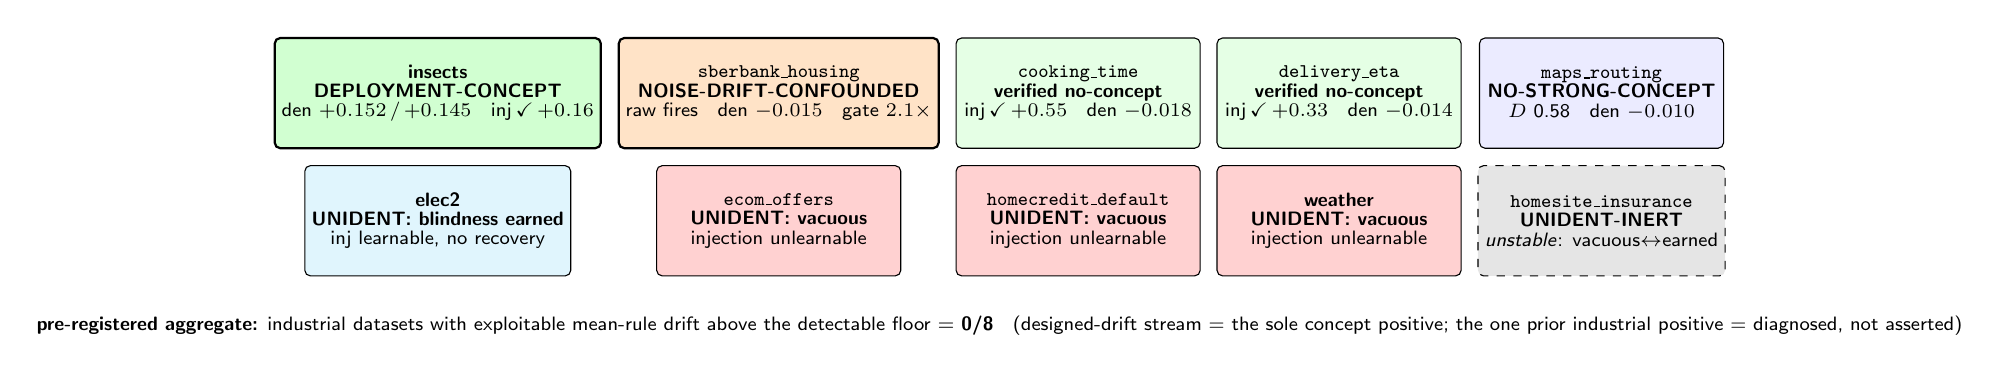
\begin{tikzpicture}[
  font=\scriptsize\sffamily,
  tile/.style={draw,rounded corners=2pt,minimum width=31mm,minimum height=14mm,align=center,inner sep=2.5pt},
  good/.style={tile,fill=green!18,thick},
  vnull/.style={tile,fill=green!10},
  warn/.style={tile,fill=orange!22,thick},
  idnull/.style={tile,fill=blue!8},
  earned/.style={tile,fill=cyan!12},
  bad/.style={tile,fill=red!18},
  unst/.style={tile,fill=black!10,dashed}
]
\matrix (m) [column sep=2mm, row sep=2mm] {
  \node[good]  {\textbf{insects}\\[-1pt]\textbf{DEPLOYMENT-CONCEPT}\\[-1pt]den $+0.152$\,/\,$+0.145$ \; inj\,\checkmark\,$+0.16$}; &
  \node[warn]  {\texttt{sberbank\_housing}\\[-1pt]\textbf{NOISE-DRIFT-CONFOUNDED}\\[-1pt]raw fires \; den $-0.015$ \; gate $2.1\times$}; &
  \node[vnull] {\texttt{cooking\_time}\\[-1pt]\textbf{verified no-concept}\\[-1pt]inj\,\checkmark\,$+0.55$ \; den $-0.018$}; &
  \node[vnull] {\texttt{delivery\_eta}\\[-1pt]\textbf{verified no-concept}\\[-1pt]inj\,\checkmark\,$+0.33$ \; den $-0.014$}; &
  \node[idnull]{\texttt{maps\_routing}\\[-1pt]\textbf{NO-STRONG-CONCEPT}\\[-1pt]$D$ 0.58 \; den $-0.010$}; \\
  \node[earned]{\textbf{elec2}\\[-1pt]\textbf{UNIDENT: blindness earned}\\[-1pt]inj learnable, no recovery}; &
  \node[bad]   {\texttt{ecom\_offers}\\[-1pt]\textbf{UNIDENT: vacuous}\\[-1pt]injection unlearnable}; &
  \node[bad]   {\texttt{homecredit\_default}\\[-1pt]\textbf{UNIDENT: vacuous}\\[-1pt]injection unlearnable}; &
  \node[bad]   {\textbf{weather}\\[-1pt]\textbf{UNIDENT: vacuous}\\[-1pt]injection unlearnable}; &
  \node[unst]  {\texttt{homesite\_insurance}\\[-1pt]\textbf{UNIDENT-INERT}\\[-1pt]\emph{unstable}: vacuous$\leftrightarrow$earned}; \\
};
\node[below=2.5mm of m,align=center,font=\scriptsize\sffamily]
  {\textbf{pre-registered aggregate:} industrial datasets with exploitable mean-rule drift above the detectable floor $=$ \textbf{0/8}
   \; (designed-drift stream = the sole concept positive; the one prior industrial positive = diagnosed, not asserted)};
\end{tikzpicture}
}
\caption{The identifiability map at a glance (Table~\ref{tab:map} is the precise record). Tile
color encodes the verdict class: green $=$ rule-change verdict or verified no-concept; amber $=$
diagnosed noise mechanism; blue $=$ identifiable null; light blue $=$ earned blindness; red $=$
certificate refused; grey (dashed) $=$ unstable across seed sets. Each tile carries its
load-bearing number (denoised staleness, exploratory\,/\,confirmatory where both exist, or
injection recovery). Color is redundant: every tile also prints its verdict.}
\label{fig:map}
\end{figure}

\begin{table}[t]
\caption{The identifiability map. Where two numbers are shown: exploratory / confirmatory.}
\label{tab:map}
\centering
\scriptsize
\setlength{\tabcolsep}{2pt}
\begin{tabular}{@{}l>{\raggedright\arraybackslash}p{0.92in}>{\raggedright\arraybackslash}p{0.78in}>{\raggedright\arraybackslash}p{0.78in}>{\raggedright\arraybackslash}p{0.55in}>{\raggedright\arraybackslash}p{0.30in}>{\raggedright\arraybackslash}p{0.40in}>{\raggedright\arraybackslash}p{1.02in}@{}}
\toprule
dataset & verdict ($=$ confirmatory) & raw & denoised & gate & $D$ & Rec. & certificate \\
\midrule
insects & \textbf{DEPLOYMENT-CONCEPT} & $+0.135$ / $+0.129$ & $\boldsymbol{+0.152}$ / $\boldsymbol{+0.145}$ & 1.24 & 0.844 & $+0.162$ & injection recovers \\
\texttt{sberbank\_housing} & \textbf{NOISE-DRIFT-CONFOUNDED} & $+0.024$ / $+0.033$ (fires) & $\boldsymbol{-0.015}$ / $\boldsymbol{-0.011}$ & \textbf{2.11 / 2.21 (fires)} & 1.000 & --- & --- (diagnosed, \S\ref{sec:diagnosis}) \\
\texttt{cooking\_time} & INJECTION-RECOVERED & $-0.011$ & $-0.018$ & 0.92 & 0.966 & $\boldsymbol{+0.546}$ & \textbf{verified no-concept} \\
\texttt{delivery\_eta} & INJECTION-RECOVERED & $-0.012$ & $-0.014$ & 0.89 & 0.999 & $\boldsymbol{+0.332}$ & \textbf{verified no-concept} \\
\texttt{maps\_routing} & NO-STRONG-CONCEPT & $-0.008$ & $-0.010$ & 1.01 & 0.578 & n/a & identifiable region \\
elec2 & UNIDENTIFIABLE & $+0.001$ & $+0.001$ & 0.66 & 1.000 & $+0.018$ & \textbf{blindness earned} (inj learnable) \\
\texttt{ecom\_offers} & UNIDENTIFIABLE & $-0.001$ & $-0.007$ & 1.25 & 1.000 & --- & \emph{vacuous}---unlearnable (0/4 fam.) \\
\texttt{homecredit\_default} & UNIDENTIFIABLE & $-0.007$ & $+0.004$ & 1.29 & 1.000 & --- & \emph{vacuous} (0/4 fam.; 80 proxies stripped) \\
weather & INJECTION-RECOVERED\,$\dagger$ & $-0.012$ & $-0.011$ & 0.93 & 0.994 & $\mathbf{+0.183}$ & 	extbf{verified no-concept} (2/3 fam.) \\
\texttt{homesite\_insurance} & UNIDENTIFIABLE-INERT & $-0.004$ & $-0.002$ & 1.14 & 1.000 & $-0.001$ & \textbf{blindness earned} (2/2 fam., stable) \\
\bottomrule
\end{tabular}

\vspace{2pt}
{\scriptsize $D$ $=$ \texttt{D\_strip}, the group-aware separability median ($D^\star = 0.96$ routes
to the injection control). Rec.\ $=$ recovered staleness of a planted rule at reference strength (2.5\,rad);
``---'' $=$ the injection was unlearnable in every signal family tried, so no recovery number is
admissible (vacuity discipline), and n/a $=$ the cell never routes to the injection control.
Recovery values move by ${<}0.01$ between seed sets on every cell. $\dagger$ weather's
reference-family rule is unlearnable in its geometry; recovery is measured under the low-variance
carrier, where it reproduces on fresh seeds ($+0.183$ / $+0.193$) and under the interaction family
($+0.083$ / $+0.078$), both also clearing the strict rule. The ``(m/n fam.)'' counts report how
many signal families were learnable and how many of those recovered, so a certificate is never
read as stronger than the class of rule change it was actually tested against.}
\end{table}

Figure~\ref{fig:map} gives the map at a glance; Table~\ref{tab:map} is the precise record. The
pre-registered aggregate reading:
\textbf{relative to the tree-ensemble class, the number of industrial datasets with exploitable
mean-rule drift above the per-dataset detectable floor is 0/8.} That count is over the eight
datasets \emph{audited}; the count over the datasets \emph{whose identifiability is certified} is
\textbf{0/5}, because \texttt{ecom\_offers} and \texttt{homecredit\_default} alone end with no
certificate---their planted probe rule is unlearnable under every signal family tried---and so
contribute no evidence in either direction. We report both numbers wherever the aggregate appears: the first is what was
pre-registered, the second is what it is worth. The only concept positive is
the designed-drift stream, where the denoised arm \emph{exceeds} the raw arm---pseudo-labels encode
the old rule cleanly once label noise is removed, the signature of genuine rule change. Two of
the four industrial blindness claims that a naive protocol would have granted end without any
earned certificate, because the planted probe rule is unlearnable in those geometries and their
top-variance features cannot carry it---a distinction invisible without the learnability gate.
The other two are settled by widening the signal family rather than by assumption: weather's
geometry carries a rule fine on its \emph{low-variance} features and the real null survives the
power certificate that follows, and \texttt{homesite\_insurance} is learnable there too and stays
unrecovered, which converts the seed-unstable label of the first reading into earned blindness. The strongest cells in the map are,
counter-intuitively, the two verified no-concept certificates: geometry demonstrably has power
($+0.55$/$+0.33$ recovery of a planted rule) and the real staleness is still null.

\paragraph{Certified is not uniform: power collapses inside the routing region.}
$D^\star = 0.96$ is a binary gate, but the injection control---a planted rule of \emph{fixed}
strength (2.5\,rad)---is recovered at very different magnitudes just inside it:
\texttt{cooking\_time} ($D = 0.966$) recovers $+0.546$, \texttt{delivery\_eta} ($D = 0.999$)
$+0.332$, Electricity ($D = 1.000$) $+0.018$, \texttt{homesite\_insurance} ($D = 1.000$) $-0.052$.
Learnability does not explain the ordering---Electricity's planted rule is the \emph{most}
learnable in the panel (in-window AUC 0.976) and still barely recovers; what collapses across $D$
is recovery, not learnability. Over every learnable injection run at decision grade the rank
correlation between $D$ and recovery is $\rho = -0.47$ ($p = 0.037$, $n = 20$); the cleanest
within-dataset contrast is Electricity itself, whose identical planted rule recovers $+0.190$ at
$D = 0.905$ under the linear probe---ten times its recovery at $D = 1.000$ under HGB. A
certificate therefore certifies that the geometry had power \emph{at this separability}, not that
power is uniform across the certified cells; the Rec.\ column of Table~\ref{tab:map} makes that
spread visible, and the threshold of \S\ref{sec:certificates} should be read as routing laid over
a continuous and steep decay rather than as a cliff.

\subsection{The diagnosis: how the instrument caught its own prior positive}\label{sec:diagnosis}

The v2-era instrument (raw arm only) had reported sberbank-housing---the panel's one regression
dataset---as its sole industrial concept positive ($+0.024$ $[+0.018, +0.030]$). The audit
constructed the noise-decay null of \S\ref{sec:battery} at matching magnitude; the v3 rerun then delivered the
diagnosis. Across window resolutions $K \in \{5, 8, 10, 12, 20\}$: the raw arm fires at $K \in \{8, 10,
12\}$ (at $K = 10$ reproducing the v2 headline \textbf{bit-for-bit}\footnote{Bit-identical at
full precision: $+0.023900573591226625$, recorded verbatim in the committed artifact.} at
$+0.0239$---the raw
pipeline's RNG stream is unchanged, so this is the \emph{same} signal reinterpreted, not a
re-measurement that happened to differ); the old window's measured noise proxy is 2.1--2.9$\times$ the
recent median at every $K$; and the \textbf{denoised arm is significantly negative at every $K$} ($-0.014$
to $-0.018$, all CIs below zero): replace the old labels with cross-fitted pseudo-labels and the
old rows \emph{help}. The rule did not change; the early labels are noisier---consistent with
2011--2012 crisis-era Russian housing prices. At $K = 20$ the injection control recovers a planted
rule ($+0.101$) through the same geometry, and at no $K$ does any rule reading yield CONCEPT.
(The diagnosis is of the minted positive; it does not exclude a residual rule change below the
floor co-occurring with the noise decay---no sub-floor claim is made in either direction.) The
diagnosis now also carries the power certificate it originally lacked. Under the strict decision
rule this cell's shadow verdict lands in the unidentifiable branch and therefore reaches the
injection stage, where a planted rule at reference strength is learnable in its geometry
(in-window $R^2$ 0.93) and recovers at $+0.086$, clearing both rules. So the negative denoised arm
is not a power failure: the same windows that fail to show rule change do show a rule change that
was put there. The primary and strict readings then say the same thing by different routes---the
minted positive was noise, and the null underneath it is informative. We are
not aware of a prior case of a drift-attribution instrument diagnosing the \emph{mechanism} of its
own earlier false positive on real data, as opposed to merely failing to replicate it.

\subsection{The class panel on real data}\label{sec:classpanel}

The decision-grade classes agree: \textbf{HGB and random-forest verdicts match operatively on 10/10
datasets} (one sub-label difference). The canaries do not---and the flip that matters is
replicated across two independent canary classes: \textbf{both the linear probe (raw $+0.023$, denoised
$+0.033$, injection recovers $+0.190$) and the MLP probe (raw $+0.007$, denoised $+0.025$) read
Electricity as DEPLOYMENT-CONCEPT} where the tree-ensemble probe reads it
unidentifiable-with-earned-blindness. Electricity is the literature's canonical concept-drift
dataset; whether a monitor confirms that reputation depends on the probe class, on identical
data. The MLP panel also illustrates why canary verdicts must not be consumed directly: on the
regression datasets its staleness estimates are numerically unstable (sberbank CI spanning $\pm 15$
z-units; weather CI width 0.5)---driven by a few divergent fits: on sberbank, three of ten seeds
land at $|\text{staleness}| > 10$ z-units while the other seven lie within $\pm 2$ (per-seed
values in the committed artifact), i.e., occasional optimization failure of the un-tuned probe
rather than signal---and no TabReD cell produces a new positive under it---the
decision-grade map is unchanged. A second canary behavior is worth reporting as a
warning: on \texttt{ecom\_offers} the linear probe fires the \emph{denoised} arm only ($+0.028$) with the raw arm
null ($-0.002$)---a denoiser-artifact channel specific to misspecified probes (the linear $\hat{g}_{\text{old}}$'s
systematic error is itself informative to the linear downstream model), reinforcing that the
denoised arm's semantics are also class-scoped.

\section{Anchors and the Sensitivity Profile}\label{sec:anchors}

The map's credibility rests on knowing what the instrument \emph{can} see. We ran it over 23
synthetic river streams (SEA/Agrawal/STAGGER/Sine/Hyperplane; no-drift / abrupt single-switch /
gradual / reoccurring variants) and all seven INSECTS variants (real sensor data, lab-controlled
temperature drift; \citealp{souza2020challenges}).

\paragraph{Monotone and single-switch rule changes fire: 9/9.} River: \texttt{agrawal\_abrupt} $+0.045$,
\texttt{agrawal\_gradual} $+0.047$, \texttt{stagger\_abrupt}, \texttt{sine\_abrupt} $+0.031$, \texttt{hyperplane\_incremental} $+0.112$ (with
the gate correctly co-flagging its noise component), \texttt{sine\_reoccur2}\footnote{Reoccurring
in name only for this lens's horizon: the stream returns to its
initial regime just in its final ${\approx}22\%$, so most evaluated back-half windows sit inside
the middle regime, whose rule is a near label-inversion of the anchor's---its recency gain is
strongly \emph{positive} ($+0.30$), the opposite of the recurring fingerprint, and
geometry-matched siblings whose middle regime is not label-inverting read ${\approx}0$
(\texttt{sine\_reoccur} $-0.003$, \texttt{sine\_reoccur3} $-0.003$).} $+0.047$. INSECTS:
gradual-balanced $+0.092$, gradual-imbalanced $+0.069$, incremental $+0.135$---in every firing cell,
denoised $\ge$ raw, and the injection positive-control recovers. Weak switches (SEA's threshold
nudge) land in the no-evidence band with consistent sign, reported with their detectable floors.

\paragraph{Recurring regimes are correctly silent---and fingerprinted.} INSECTS abrupt variants
(oscillating temperature) read \emph{negative} staleness (old data helps: $-0.070$, $-0.027$) with
\textbf{negative recency gain} ($-0.058$, $-0.023$): the window adjacent to the test predicts it \emph{worse}
than the oldest window does. Negative recency is impossible under one-way drift; it is the
signature of a regime that has returned. The same pattern holds across river's reoccurring
cells and INSECTS incremental-reoccurring---three independent confirmations. This is a scope
statement, not a defect: the lens answers the deployment question (``does old data harm a model
trained today?''), and when old regimes recur, old data genuinely does not harm---recency does.
A monitor built on this lens will not \emph{detect} recurring concept drift; it will correctly tell
you old data is safe to keep, and its negative-recency flag tells you why. On the audited panel
that flag is silent: every industrial cell reads recency gain $\ge 0$ (from $+0.000$ on
\texttt{maps\_routing} to $+0.325$ on sberbank-housing), nowhere near the recurring signature
($-0.023$ to $-0.058$ on the oscillating streams). This is deliberately a scoped statement:
negative recency certifies recurrence only at scales that dominate the evaluation horizon---our
own \texttt{sine\_reoccur2} anchor shows a late-returning regime (final ${\approx}22\%$)
reading recency $+0.30$---and drift at sub-window timescales is averaged away
(\S\ref{sec:discussion}, Limitation 2). The silent flag therefore rules out horizon-dominating
recurrence on the audited panel; it says nothing about late, brief, or sub-window-periodic
returns (intraday or day-of-week seasonality included), which remain uncovered by this check.

\paragraph{Calibration of the no-evidence band.} Two of five no-drift anchor streams produce
``CI-significant'' sub-floor denoised positives at 1/10--1/20 of the decision floor---seed-level
CIs on overlapping subsamples are anti-conservative at tiny magnitudes. Accordingly, the
sub-floor band is read as \emph{no evidence} everywhere in this paper, a calibration the anchor suite
forced and the pre-registration records.

\paragraph{Malware (EMBER).} On 2018-dense monthly windows the cell is certificate-grade:
DEPLOYMENT-DECAY-COVARIATE with $D = 0.834$ (identifiable---the null carries full weight), raw
staleness $-0.008$ $[-.009, -.007]$ (old data helps), denoised $-0.004$, gate quiet, recency gain
$+0.031$ above the floor, detectable floor 0.0013. (``Certificate-grade'' refers to
identifiability, not magnitude: the mechanism label rests on the above-floor recency gain and
the significantly negative staleness; the no-evidence-band discipline governs sub-floor
\emph{positives} and is not invoked here.) Malware's temporal degradation
\citep{pendlebury2019tesseract} is real and recency-recoverable, but it is coverage-driven---new
families appear; old labels do not rot---and the deployment lens draws exactly that distinction:
keep the old data, expect decay anyway, retrain for coverage. (A full-history windowing over 126
sparse months gives the same null at lower power, and a mis-windowed attempt on 19-row windows
correctly refused to emit a verdict.)

\paragraph{The WhyShift bridge (ACS across years).} WhyShift reported $Y \mid X$-shifts as prevalent on
ACSIncome across \emph{states}; running the instrument on the same task across \emph{years} (California,
2014--2018, yearly windows, 10 seeds) yields the map's best-powered null: NO-STRONG-CONCEPT with
raw $-0.008$ and denoised $-0.007$ (both CIs negative---old years help), gate quiet, $D = 0.515$
(the years are barely separable in feature space---negligible covariate movement, fully
identifiable), recency $\approx 0$, and a detectable floor of 0.0008. The same task whose spatial axis
exhibits prevalent $Y \mid X$-shift is temporally quiet over five years---the axis, not just the
dataset, determines the shift type. (An overlap-based decomposition run on the same cell
agrees: within-overlap gap $-0.009 \approx$ placebo $-0.008$ at cov-AUC 0.68---Appendix~\ref{app:rebuttal}.) The cell also passes a real-data analogue of the
prior-shift control: the fixed \$50k income threshold under inflation produces a monotone
positive-rate ramp ($0.36 \to 0.42$), and the instrument does not misread that prior drift as
concept. (Scope: one state, five pre-COVID years; a multi-state extension is future work.)

\section{Discussion}\label{sec:discussion}

\paragraph{What a practitioner gets.} Raw staleness answers ``does old data hurt?''; the repaired
instrument answers ``\emph{why}, and what to do about it,'' with a decision rule per cell: a denoised
fire inside the envelope $\Rightarrow$ the rule changed for your model class---old labels are poison,
retrain recent-only or add temporal structure; a raw fire with the gate on $\Rightarrow$ your labels' noise
profile drifted---old rows are \emph{reusable} via self-training (the denoised arm is literally that
remedy, measured); nulls with a recovery certificate $\Rightarrow$ retraining chases coverage, not rule
change; negative recency $\Rightarrow$ regimes recur---retention, not recency, is your friend; vacuous or
unstable certificates $\Rightarrow$ do not let a monitor speak about this dataset's drift type at all.

\paragraph{What the map means, and does not.} The 0/8 aggregate does \emph{not} say concept drift is absent
from industrial tabular ML: \textbf{two of the eight cells are certificate-less} (their injections
are unlearnable in every signal family tried), and exactly one of the eight is
blind-but-certified (\texttt{homesite\_insurance}); Electricity, the panel's other earned
blindness, is not one of the industrial eight. The aggregate is therefore 0/8 audited but 0/5 informative; blindness is
not absence, and neither is vacuity. It says something narrower and, we argue, more useful: on the
benchmark the field uses to argue for time-aware tabular architectures, \textbf{no measurable
mean-rule drift exists for the model class that dominates those benchmarks, and every apparent
counterexample so far has dissolved under controls}---the last one into label-noise decay,
diagnosed rather than asserted. The burden of proof for ``temporal architecture X exploits
concept drift on TabReD-like data'' should now include an identifiability certificate.

\paragraph{Limitations.} (1) Verdicts are tree-ensemble-scoped; we show this scoping is necessary, not
that it is sufficient for every deployed system. The panel's neural probe (a two-layer MLP)
fails the separation battery and is classified a canary (\S\ref{sec:classmatrix}); modern deep tabular
architectures (FT-Transformer-class, at production scale) remain untested---extending the panel
is the clearest next step, with the battery as the pre-registered entry bar any such probe must
pass before its drift verdicts are trusted. (1b) \textbf{Scale.} The probe trains on $N \le 6{,}000$ rows
per arm; industrial models train on orders of magnitude more. A rule change exploitable only at
much larger $N$ is invisible here, so every $\delta$ bound and the 0/8 (0/5 certified) aggregate are statements \emph{at probe
scale}. A first $\delta(N)$ sweep (Appendix~\ref{app:rebuttal}) raises the arm cap to the
window-geometry ceiling ($N \approx$ 14k--24k, up to $4\times$ the headline scale) on the three
largest null cells: every verdict is unchanged and no reading trends toward the floor.
Production-scale $N$ beyond that remains future work, and we flag rather than dismiss the
possibility that the map changes there. Scale enters a second way: because the arms differ in size
($N$ vs $2N$), a sample-size gain is folded into every staleness reading. Measured directly
(Table~\ref{tab:sizeterm}) it is negligible on binary cells but reaches 61\% of the decision floor
on regression, which effectively raises the detectable floor on the map's five regression cells;
we report their nulls with that displacement stated rather than absorbed.
(2) $K = 10$ rolling windows with a fixed early
anchor: drift at time scales far below the window width is averaged away (the injection control
partially measures this---its recovery varies with $K$), and the TabReD map covers the train
segments of the official splits---though the full-span audit of Appendix~\ref{app:rebuttal}, B.4
crosses that gap and moves no verdict. (3) The single robust positive
is lab-designed drift; we found no naturally occurring industrial positive to calibrate
magnitude against---that is the map's finding and its weakness simultaneously. (4) The envelope
constant (4.7) is calibrated on Gaussian noise families; heavy-tailed label noise inherits only
the abstention discipline, not the exact boundary. (5) TabReD is curated to be temporally
splittable; external validity to industrial data at large is an inductive step we flag rather
than take. (6) The injection certificates were calibrated on a single reference family,
and the sweep that was owed here has now been run (Appendix~\ref{app:rebuttal}, B.5): power is
\textbf{certified against low-variance rotations and against interaction-borne rules}, and
\textbf{disconfirmed against subpopulation-local rule change}---on weather, a planted
subpopulation-local rule is comfortably learnable in-window ($R^2$ 0.560) and still fails to
recover ($-0.050$), reproducing on confirmatory seeds, while the same geometry recovers
low-variance ($+0.128$) and interaction ($+0.046$) rules. ``Verified no-concept'' therefore
carries an explicit family denominator throughout \S\ref{sec:results}, and the relativity of
certificates is a measured property rather than a caveat.

(7) \textbf{The probe is blind to rule change that moves a threshold without reordering.} We
tested the instrument against an externally documented rule change: the ACA Medicaid expansion,
which Pennsylvania implemented on 2015-01-01 and Texas never adopted, on the ACS public-coverage
task over 2014--2018 (Appendix~\ref{app:rebuttal}, B.6). The expansion lifted Pennsylvania's
positive rate from 0.234 to 0.306 with the step at the implementation year, while Texas stayed
flat within 0.2 points. The probe read \textbf{both states null}, in a fully identifiable regime
($D = 0.53$) and at the tightest detectable bound anywhere in this paper ($\delta = 0.00083$)---so
this is not an underpowered null but a confident zero, which makes the miss sharper rather than
softer. The mechanism was registered before the run and is confirmed by it: our binary score is
AUC, which is rank-based, and an eligibility threshold can move a large mass of people across a
decision boundary without reordering anyone. Measured on the same rows with a proper score, the
treatment-versus-control separation widens from $3.1\times$ under AUC to $6.3\times$ under Brier,
$6.6\times$ under log-loss and $15\times$ under a rule-movement divergence. But it does not become
large: every reading stays below the decision floors of both instruments, and the control state
also returns placebo-significant gaps, so only the treatment/control \emph{ratio} is
interpretable. The honest statement is therefore not ``the metric explains the miss'' but ``the
metric compresses the signal six- to sevenfold, and even uncompressed this policy change sits
under our floor.'' Two consequences follow. Every null in \S\ref{sec:map} should be read as scoped
to a rank-based score, which is the right scope for a ranking or triage system and the wrong one
for the fixed-threshold eligibility systems this very task represents. And the decision floor of
0.02, calibrated on planted effects and no-drift anchors, is larger than a real population-scale
policy rule change---recorded as a measured criticism of that constant in
Appendix~\ref{app:constants} rather than acted on, since changing a pre-registered threshold after
seeing results is what this paper argues against.

\paragraph{On process.} This project's ledger records nine positive findings that dissolved under
scrutiny before the present result; the ninth dissolution is \S\ref{sec:diagnosis}, and it is the only one the
measuring instrument itself diagnosed. The methodological claim we stand behind is that the
combination that finally produced a stable result---executed adversarial nulls before real-data
claims, pre-registered cascades with commit-timestamped predictions, confirmatory fresh-seed
replication, certificates instead of assumptions, and canary probes---is cheap relative to the
cost of the dissolutions it prevents, and we release the audit trail as part of the artifact.

\paragraph{Future work.} Multi-state and post-2019 extensions of the ACS bridge (\S\ref{sec:anchors}); class-invariance
conditions for the denoised arm (when does a probe family admit \emph{any} sound staleness
reading?); a $\delta(N)$ scaling study; and porting the certificate protocol to streaming monitors,
where the recurring-regime fingerprint (negative recency) is directly actionable.

\section{Reproducibility}\label{sec:repro}

% SUBMISSION TODO: replace with the anonymized mirror link (e.g. anonymous.4open.science),
% preserving commit history — the commit timeline is part of the pre-registration argument.
Everything is in one repository, linked in anonymized form for review. The instrument is a
single sklearn-only script
(\texttt{scripts/run\_deployment\_decay.py}); every stochastic step is seeded, and every output artifact
embeds its commit hash, argv, library versions, and UTC timestamp. That stamping is not ceremony,
and we can say so from an incident rather than from principle: one battery run was executed under
the wrong interpreter because the shell prompt announced the intended conda environment while
\texttt{PATH} still resolved to an unrelated project's virtualenv. The verdicts passed, so nothing
on screen looked wrong; the artifact's recorded library versions did not match the environment the
real-data runs use, and that mismatch is the only thing that caught it. Had the run been trusted, a
gate certified in one environment would have licensed measurements in another---the precise failure
the pre-registration had already logged once before and repaired (\S\ref{sec:battery}). Every
subsequent run invokes the interpreter by absolute path and asserts its version before doing
anything else.
\paragraph{Compute.} Every run in the paper is CPU-only---the instrument and all probe classes
are scikit-learn models; no GPU is used anywhere---executed single-node on one shared multicore
Linux server (Python 3.11.15, scikit-learn 1.9.0, NumPy 2.4.6; the environment freeze is
committed). Wall-clock is reconstructable from the committed phase logs: the main pre-registered
phases ran phase-parallel in ${\approx}17$\,h on one calendar day, the model-class panel adds
${\approx}2$\,h, and the optional cells (EMBER, the ACS bridge, canary reruns) ${\approx}13$\,h
across two further days; no single dataset cell exceeds a few CPU-hours. Per-source data access
and license terms are tabulated in Appendix~\ref{app:licenses}. The synthetic battery is
byte-reproducible (re-running \texttt{-{}-synth} regenerates the committed artifact SHA-identical on the
same environment), and the raw arm's RNG stream is stable across instrument versions (the v2
headline number reproduces bit-for-bit under v3, which is what makes \S\ref{sec:diagnosis} a reinterpretation
rather than a re-roll). The pre-registration (\texttt{PREREG\_DEPLOYMENT\_V2.md}) freezes thresholds,
cascade, seed protocol, and aggregate reading, with results appended as read-only sections whose
ordering is enforced by the git history; all server runs are reproduced by one resumable driver
(\texttt{scripts/run\_prereg\_phases.sh}, marker-based, phase-parallel), and the environment freeze of
the machine that produced the headline numbers is committed. One deviation from the registered
procedure is disclosed: the family sweep specified a human checkpoint after its implementation
control, and the batch that ran it computed all four signal families before that checkpoint was
read, so the gate became a read-time filter rather than an execution-time one. No family was
excluded in the event---the control recovered in all four---but the order differed from what was
committed, and the record says so. Data access: TabReD requires
Kaggle authentication and per-competition rule acceptance; elec2 fetches from OpenML; INSECTS
and the river panel install via \texttt{river}; EMBER-2018 downloads from its public archive and is
parsed by a dependency-free adapter. Exact cross-version bit-reproducibility of
HistGradientBoosting across sklearn releases is \emph{not} claimed; verdict-level stability across
seed sets and across HGB/RF is (10/10 and 10/10, \S\ref{sec:map}).

\bibliography{main}
\bibliographystyle{tmlr}

\appendix
\section{Data access and licenses}\label{app:licenses}

Verified against each distributor at the time of writing (Table~\ref{tab:licenses}).

\begin{table}[h]
\caption{Data access paths and license terms, per source.}
\label{tab:licenses}
\centering
\footnotesize
\begin{tabular}{@{}>{\raggedright\arraybackslash}p{1.75in}>{\raggedright\arraybackslash}p{2.05in}>{\raggedright\arraybackslash}p{2.35in}@{}}
\toprule
source & access path in the pipeline & license / terms \\
\midrule
TabReD (8 industrial datasets) & Kaggle, via the TabReD preprocessing tooling & per-competition Kaggle rules (acceptance required); TabReD tooling Apache-2.0 \\
Electricity (elec2) & OpenML dataset 151 & listed ``Public'' by OpenML \\
INSECTS (7 variants) & fetched through the \texttt{river} package & \texttt{river} BSD-3-Clause; dataset introduced by \citet{souza2020challenges} \\
river synthetic streams (SEA / Agrawal / STAGGER / Sine / Hyperplane) & generated by \texttt{river} & BSD-3-Clause \\
EMBER-2018 & public archive download; parsed by our dependency-free adapter & data files MIT (the ember \emph{code} is AGPL-v3 and is not used) \\
ACS (folktables bridge) & \texttt{folktables} & folktables MIT; ACS PUMS is public U.S.\ Census Bureau data \\
\bottomrule
\end{tabular}
\end{table}

\section{Robustness, hardening, and one external test}\label{app:rebuttal}

Both checks were run after the pre-registered audit froze, with the instrument, cascade, and
thresholds unchanged (commit-stamped artifacts); they are robustness checks, not pre-registered
cells.

\paragraph{B.1 $\delta(N)$: the map does not move toward the floor as $N$ grows.} The probe's
headline scale is $N \le 6{,}000$ (\S\ref{sec:discussion}, Limitation 1b). We re-ran the three
largest null cells with the arm cap swept over $\{1{,}500,\ 24{,}000,\ 96{,}000\}$ (10 seeds
each). Window geometry bounds the realizable arm size ($N = \min(|\text{recent}|, |\text{old}|,
\text{cap})$, and $|\text{window}| \approx n/K$), so the realized ceilings are ${\approx}17{,}200$
on \texttt{homecredit\_default} (the 96{,}000 cap realizes the same $N$), 24{,}000 on weather
(cap-bound), and ${\approx}14{,}300$ on \texttt{maps\_routing}. Verdicts are unchanged at every
$N$, and nothing trends toward the 0.02 floor (Table~\ref{tab:deltaN}). Raw staleness is
significantly \emph{negative} (old data helps) at every $N$ on all three cells; the one
sub-floor positive (homecredit's denoised arm) sits at a quarter of the decision floor, is flat
across an $11\times$ range of $N$, and shrinks at the top of the range; weather's denoised arm
converges to ${\approx}0$ from below. The injection certificates reproduce (homecredit/weather
planted rules remain unlearnable---vacuous; maps identifiable). Scope unchanged: $K = 10$ window
geometry caps realizable $N$ at ${\approx}$14k--24k here, so production-scale $N$ beyond that
remains untested.

\begin{table}[h]
\caption{$\delta(N)$ sweep on the three largest null cells (10 seeds; rows at $N = 6{,}000$ are
the main-audit values of Table~\ref{tab:map}).}
\label{tab:deltaN}
\centering
\footnotesize
\setlength{\tabcolsep}{3.5pt}
\begin{tabular}{@{}llll l@{}}
\toprule
cell & realized $N$ & raw staleness & denoised & verdict \\
\midrule
\texttt{homecredit\_default} & 1{,}500 & $-0.015$ $[-.018, -.012]$ & $+0.007$ $[+.005, +.008]$ & UNIDENT (vacuous)---unchanged \\
\texttt{homecredit\_default} & 6{,}000 & $-0.007$ & $+0.004$ & unchanged \\
\texttt{homecredit\_default} & ${\approx}17{,}200$ (cap 24k) & $-0.013$ $[-.016, -.011]$ & $+0.006$ $[+.004, +.007]$ & unchanged \\
\texttt{homecredit\_default} & ${\approx}17{,}200$ (cap 96k) & $-0.010$ $[-.012, -.009]$ & $+0.005$ $[+.003, +.006]$ & unchanged \\
weather & 1{,}500 & $-0.017$ $[-.019, -.015]$ & $-0.022$ $[-.024, -.020]$ & unchanged \\
weather & 6{,}000 & $-0.012$ & $-0.011$ & unchanged \\
weather & 24{,}000 & $-0.005$ $[-.006, -.005]$ & $-0.002$ $[-.002, -.002]$ & unchanged \\
\texttt{maps\_routing} & 1{,}500 & $-0.009$ $[-.010, -.009]$ & $-0.017$ $[-.017, -.016]$ & NO-STRONG-CONCEPT \\
\texttt{maps\_routing} & 6{,}000 & $-0.008$ & $-0.010$ & unchanged \\
\texttt{maps\_routing} & ${\approx}14{,}300$ (cap 24k) & $-0.008$ $[-.009, -.008]$ & $-0.008$ $[-.009, -.008]$ & unchanged \\
\bottomrule
\end{tabular}
\end{table}

\paragraph{B.2 Cross-lens agreement where overlap holds.} On the two cells of the map whose
separability leaves an overlap-based decomposition applicable (\texttt{maps\_routing},
$D = 0.58$; the ACS bridge, $D = 0.515$), we ran the WhyShift-style within-overlap concept
decomposition (ess-gated) next to the deployment lens. The two instruments agree
(Table~\ref{tab:crosslens}): where overlap holds, the overlap lens and the deployment lens
return the same verdict; the instrument disagreements this paper documents
(\S\ref{sec:instrument}--\ref{sec:validation}) arise precisely where overlap fails---which is
why verdicts must carry certificates.

\begin{table}[h]
\caption{Cross-lens agreement on the overlap-valid cells (Appendix B.2).}
\label{tab:crosslens}
\centering
\footnotesize
\setlength{\tabcolsep}{4pt}
\begin{tabular}{@{}>{\raggedright\arraybackslash}p{1.72in}>{\raggedright\arraybackslash}p{1.55in}>{\raggedright\arraybackslash}p{1.42in}>{\raggedright\arraybackslash}p{1.32in}@{}}
\toprule
cell & deployment lens & within-overlap gap [CI] & note \\
\midrule
\texttt{maps\_routing} (full, 986 feats) & NO-STRONG-CONCEPT (den $-0.010$) & $-0.003$ $[-.004, -.002]$ & measurable 5/5 seeds, ESS 93\% \\
\texttt{maps\_routing} (sparse MI@5/10/20/50) & unchanged & $-0.005 \ldots -0.005$, all ${\approx}0$ & measurable under every representation \\
ACS CA 2014$\to$2018 & NO-STRONG-CONCEPT (den $-0.007$) & $-0.009$ (placebo $-0.008$) & cov-AUC 0.68; gap $\approx$ placebo \\
\bottomrule
\end{tabular}
\end{table}

\paragraph{B.3 The sample-size term, measured rather than argued.} Staleness compares a model
trained on $N$ recent rows against one trained on $2N$ (recent $\cup$ old), so the observed
difference mixes two effects: the \emph{gain} from doubling the training set, which pushes
staleness negative regardless of drift, and the \emph{harm} from contradicting old labels, which
pushes it positive. Only the sum is observed. A red-team objection holds that every reported
staleness---and therefore every $\delta$---is displaced by the first term. Earlier versions of
this work answered from a bias sweep recorded in prose only; the instrument now emits per-arm
\emph{absolute} scores, so the term is directly measurable on the battery cells where the rule is
fixed \textbf{and} the old rows are drawn from the same distribution as the recent ones, which
makes the observed difference the size term and nothing else.

\begin{table}[h]
\caption{The N-vs-2N sample-size term, measured on fixed-rule same-distribution battery cells.}
\label{tab:sizeterm}
\centering
\scriptsize
\setlength{\tabcolsep}{4pt}
\begin{tabular}{@{}llccc>{\raggedright\arraybackslash}p{1.35in}@{}}
\toprule
battery cell & task & recent $\to$ recent $\cup$ old & size term & vs.\ floor & per-window ($n = 25$) \\
\midrule
\texttt{synth\_stable} & binclass (AUC) & $0.9895 \to 0.9902$ & $\mathbf{+0.00074}$ & 4\% & SD 0.0016, sign mixed \\
\texttt{synth\_covariate} & binclass (AUC) & $0.9577 \to 0.9583$ & $+0.00064$ & 3\% & SD 0.0019, sign mixed \\
\texttt{synth\_covariate\_mild} & binclass (AUC) & $0.9631 \to 0.9665$ & $+0.00340$ & 17\% & SD 0.0033 \\
\texttt{synth\_reg\_stable} & regression (z-RMSE) & $-0.1343 \to -0.1222$ & $\mathbf{+0.01212}$ & \textbf{61\%} & SD 0.0048, \textbf{all 25 positive} \\
\bottomrule
\end{tabular}
\end{table}

Two readings, and we state the unfavourable one first. \textbf{On regression the term is real and
large}: 61\% of the decision floor, positive in every one of 25 windows, so it is not a
single-window artifact. A regression cell whose true rule-change harm were $+0.012$ would be
observed at ${\approx}0$ and read as a null. The detectable floor on the regression cells of the
map (\texttt{sberbank\_housing}, \texttt{cooking\_time}, \texttt{delivery\_eta},
\texttt{maps\_routing}, weather) is therefore effectively raised by roughly this amount, and their
nulls should be read with that displacement in mind (\S\ref{sec:discussion}, Limitation 1b).
\textbf{On binary classification the term is negligible}---3--4\% of the floor---but with an
important caveat we do not want to gloss: the battery's binary cells sit at AUC ${\approx}0.99$,
close enough to the ceiling that the size gain is compressed, and the industrial binary cells do
not sit there. The binary bound therefore does not transfer as measured. Per-arm absolutes are now
emitted on every run, so the same quantity will be measured directly on the industrial panel at
its next execution rather than argued from the battery.

\paragraph{B.4 The deployment gap: the map does not move across it.} The main map covers the
train segments of TabReD's official temporal splits (\S\ref{sec:discussion}, Lim.~2). We re-ran
all eight cells with train, validation and test concatenated on the shared normalised timestamp,
so the windows cross the held-out gap the official split withholds, on exploratory and then
confirmatory seeds (\textbf{8/8 identical verdicts}). No industrial cell fires CONCEPT across the
gap, so the aggregate is not re-scoped to train segments. Three cells move in ways worth recording
rather than burying. \texttt{sberbank\_housing}'s raw arm no longer clears the floor over the
longer span ($+0.006$ raw, $-0.022$ denoised), so the noise diagnosis of
\S\ref{sec:diagnosis} is scoped to the train segment. \texttt{cooking\_time}'s separability
\emph{falls} to $D = 0.927$, below the gate and against our expectation that a longer span would
raise it, leaving an identifiable null that needs no certificate. And
\texttt{homecredit\_default}'s denoised arm reads $\mathbf{+0.018}$---89\% of the decision floor
and the largest positive-direction number anywhere in this paper---with a certificate that is
\emph{earned} rather than refused here, so it reads as ``measured and under the floor'' rather
than ``not measured''. \texttt{homesite\_insurance} likewise moves from unstable to earned;
\texttt{delivery\_eta}, \texttt{maps\_routing}, \texttt{ecom\_offers} and weather are unchanged.

\paragraph{B.5 Family $\times$ carrier: what the certificates are certified against.} The
reference injection plants a rotation on the two highest-variance features. Because three of the
four rule geometries we wanted to test would otherwise have inherited that same carrier---and the
diagnosed cause of injection-vacuity on ecom/homecredit/weather is precisely those columns' heavy
tails---the sweep crosses rule geometry with carrier. An implementation control on a
designed-drift stream recovers under all four combinations ($+0.201$ / $+0.211$ / $+0.156$ /
$+0.077$), so a non-recovery below is a property of the cell, not of the code.

\begin{table}[h]
\caption{Recovered staleness by rule geometry $\times$ carrier. ``vac'' $=$ injection unlearnable,
so no recovery number is admissible.}
\label{tab:famsweep}
\centering
\scriptsize
\setlength{\tabcolsep}{4pt}
\begin{tabular}{@{}lccccl@{}}
\toprule
cell & topvar@hi & lowvar@lo & interaction@lo & subpop@lo & reading \
\midrule
\texttt{cooking\_time} & $+0.546$ & $+0.467$ & $+0.357$ & $+0.131$ & verified, 4/4 \
\texttt{delivery\_eta} & $+0.332$ & vac & $+0.274$ & vac & verified, 2/2 learnable \
elec2 & $+0.018$ & $-0.003$ & $-0.001$ & $-0.002$ & blindness earned, 4/4 \
\texttt{homesite\_insurance} & vac & $-0.001$ & vac & $-0.003$ & blindness earned, 2/2 learnable \
weather & vac & $\mathbf{+0.183}$ & $\mathbf{+0.083}$ & learnable, $\mathbf{-0.009}$ & verified, 2/3 learnable \
\texttt{ecom\_offers} & vac & vac & vac & vac & no certificate \
\texttt{homecredit\_default} & vac & vac & vac & vac & no certificate \
insects (pos.\ control) & $+0.162$ & $+0.265$ & $+0.229$ & $+0.047$ & recovers, 4/4 \
\bottomrule
\end{tabular}
\end{table}

Two results carry beyond bookkeeping. First, weather's reference-family rule is unlearnable in its
geometry (in-window $R^2$ $-0.022$) while a low-variance rule is learnable at $R^2$ 0.674 and
recovers---so a cell that a single-family protocol would have left uncertified is certified once
the carrier is widened, which is how the certified count reaches 5 rather than 4. Second, and in
the other direction: on the full-span variant of the same cell a subpopulation-local rule is
comfortably learnable ($R^2$ 0.560, far from the 0.20 gate) and still fails to recover
($-0.050$), reproducing on confirmatory seeds, while low-variance ($+0.128$) and interaction
($+0.046$) rules recover through the identical windows. The relativity of certificates is
therefore not a caveat we assert but a boundary we measured: this instrument has power against
rules carried by feature \emph{directions} and none against rules carried by \emph{subpopulation
membership}.

\paragraph{B.6 An externally documented rule change the probe does not see.} The ACA Medicaid
expansion gives a rule change whose date and scope are fixed outside the data and whose adoption
differs by state, so treatment and control exist in the same task, the same years and the same
instrument. Pennsylvania implemented on 2015-01-01; Texas had not adopted through 2018. On the ACS
public-coverage task (folktables, 2014--2018, yearly windows) the design lands in the data:
Pennsylvania's positive rate moves $0.234 \to 0.268 \to 0.293 \to 0.305 \to 0.306$ with the step
at the implementation year, while Texas stays within 0.183--0.185 throughout.

\begin{table}[h]
\caption{The probe on a documented rule change and its control.}
\label{tab:acs}
\centering
\scriptsize
\setlength{\tabcolsep}{5pt}
\begin{tabular}{@{}lcccccc@{}}
\toprule
 & verdict & raw & denoised & recency & $D$ & $\delta$ \
\midrule
Pennsylvania (treated) & NO-STRONG-CONCEPT & $-0.011$ & $-0.009$ & $\mathbf{+0.009}$ & 0.534 & $\mathbf{0.00083}$ \
Texas (control) & NO-STRONG-CONCEPT & $-0.015$ & $-0.011$ & $-0.001$ & 0.523 & 0.00200 \
\bottomrule
\end{tabular}
\end{table}

Both null. The one arm that separates them is recency gain, positive and CI-excluding-zero on the
treated state and indistinguishable from zero on the control---directionally right, and still
below the floor, so the verdict does not move. The null survives removing the default row
thinning, and the model-class panel moves three of six labels to the sub-floor band without
changing any reading (the control's linear-probe sub-floor value is in fact \emph{larger} than the
treated state's, so nothing can be claimed from that panel).

Re-measuring the same rows with proper scores localises part of the miss. Using the within-overlap
lens of B.2 on a clean pre/post pair (2014 vs 2018), with a permutation placebo and 15 seeds, the
treatment-versus-control separation of the placebo-corrected gap is $3.1\times$ under AUC,
$6.3\times$ under Brier, $6.6\times$ under log-loss and $15\times$ under a rule-movement
divergence; Pennsylvania is metric-invariant (all four positive) and Texas is not. An independent
run of the same lens family reproduces the temporal contrast ($+0.021$ vs $+0.003$). But the
effect does not become large: every value stays below both instruments' decision floors, and the
control returns placebo-significant gaps of its own, so only the ratio is interpretable. What we
can conclude is bounded accordingly---the rank-based score compresses this signal six- to
sevenfold, and uncompressing it still leaves the change under our floor. The corresponding scope
statement and the criticism this implies for the floor constant are in \S\ref{sec:discussion}
(Lim.~7) and Appendix~\ref{app:constants}.

\section{Decision constants: calibration sources and validity}\label{app:constants}

Every decision constant in the cascade, with where it was calibrated and where it stops being
valid (Table~\ref{tab:constants}). The instrument ports to a new domain by re-running this
calibration recipe (the battery of \S\ref{sec:battery} plus the no-drift anchors of
\S\ref{sec:anchors}), not by reusing the numbers.

\begin{table}[h]
\caption{Decision constants: value, role, calibration source, and validity.}
\label{tab:constants}
\centering
\scriptsize
\setlength{\tabcolsep}{3pt}
\begin{tabular}{@{}>{\raggedright\arraybackslash}p{0.78in}>{\raggedright\arraybackslash}p{0.72in}>{\raggedright\arraybackslash}p{1.22in}>{\raggedright\arraybackslash}p{1.62in}>{\raggedright\arraybackslash}p{1.62in}@{}}
\toprule
constant & value & role & calibrated on & validity / outside behavior \\
\midrule
decision floor & 0.02 & CONCEPT magnitude bar, shared across AUC / accuracy / z-scored $-$RMSE & battery concept magnitudes (planted effects 10--27$\times$ the floor); per-metric rescaling moves no cell (\S\ref{sec:battery}) & sub-floor CI-positives $=$ no-evidence band, calibrated on no-drift anchors (2/5 land at 1/10--1/20 of the floor). \textbf{Measured criticism:} larger than a real population-scale policy rule change (\S\ref{sec:discussion}, Lim.~7)---see note below \\
noise gate & 1.5 & label-noise-drift flag (old proxy / recent median) & stable synthetic controls read 0.75--0.99; noise-drift cells read 3.5--3.9 & every real-data value falls below 1.5 or in 2.0--2.9---nowhere near the envelope edge \\
envelope & 4.7 & denoiser validity boundary; abstain above & measured on fixed-rule nulls: $+0.014$ at ratio 4.72, $+0.026$ at 5.71 (crosses the floor) & Gaussian noise family only; heavy tails inherit the abstention discipline, not the number (\S\ref{sec:discussion}, Lim.~4) \\
$D^{\ast}$ & 0.96 & separability routing to the injection control & group-aware, size-matched repairs (duplicates 0.994$\to{\approx}$0.50; shuffle-$D$ 0.94$\to$0.50) & a routing statistic, never support overlap; $D \ge D^{\ast}$ concludes nothing by itself \\
learnability gates & AUC 0.65 / $R^2$ 0.20 / acc maj.$+$0.10 & injection-certificate validity & executed junk-geometry control (in-window AUC 0.506 $\to$ vacuous) vs learnable control (0.964 $\to$ recovery $+0.195$) & unlearnable $\Rightarrow$ certificate refused for that family---vacuity, not blindness \\
injection strength & 2.5 rad & reference rotation magnitude & clears the floor on learnable geometry (recoveries $+0.16$ to $+0.55$) & family sweep executed (Appendix~\ref{app:rebuttal}, B.5): certified vs low-variance and interaction rules, \textbf{disconfirmed vs subpopulation-local} (\S\ref{sec:discussion}, Lim.~6) \\
seed protocol & 10 (0--9) $+$ conf.\ (100--109); battery 5 & power and stability & battery effects at 10--27$\times$ the floor make 5 a sufficient pass/fail gate & verdicts that move between seed sets are barred (unstable) \\
\bottomrule
\end{tabular}
\end{table}

\paragraph{Note on the decision floor (recorded, not acted on).} The pre-registration specified
that if the floor turned out to exceed a real policy-scale rule change, that fact would be logged
here as a measured criticism of the constant. It did. The ACA Medicaid expansion moved
Pennsylvania's public-coverage rate by 7.2 points on the audited population, with the step at the
implementation year, and produced no reading above 0.02 under any metric or probe class we ran
(\S\ref{sec:discussion}, Lim.~7; Appendix~\ref{app:rebuttal}, B.6). The floor was calibrated on
planted effects at 10--27$\times$ its value and on no-drift anchors at 1/10--1/20 of it, and this
event falls in the gap between those two calibration regimes---which is precisely where a decision
constant is least defensible. We do not change it: altering a pre-registered threshold after
seeing the result it would have flipped is the practice this paper argues against. What follows
instead is a scope statement---every CONCEPT verdict in this paper means ``at or above a magnitude
that a large real policy change does not reach''---and a concrete recalibration target for anyone
porting the instrument: anchor the floor on a documented rule change in the target domain, not
only on planted rotations and null streams.

\end{document}
